\chapter{DVS} \label{ch:DVS}

\section{Abstract}
The Dynamic Vision Sensor as used in \citet{Belbachir01} and \citet{Belbachir02} is an asynchronous sensor that detects changes in intensity over time and sends the pixel address as event. As there is no similar sensor available, the Ramstix is used to extract similar events from a stereo camera. This reduces the amount of data that needs to be processed. A disparity map can be calculated from the extracted events with much lower resource requirements than for typical stereo vision which makes this approach perfect for an embedded systems project. 

\section{Background}
The above mentioned sensor consists of an array of 128*128 pixels which detect intensity changes over time. Every pixel works asynchronously and can send two different events signaling an increase or decrease in intensity at a certain position. Each sent event consists of the event polarity and the pixel position. The asynchronous output leads to a high temporal resolution while the amount of data compared to a whole frame from a typical camera is notably decreased. Using this sensor for stereo vision like in \citet{Belbachir01} makes for a quite efficient embedded system. 

The outline of the stereo vision algorithm in \citet{Belbachir01} can be seen in figure \ref{fig:DVS_stereo}. The asynchronous events enter the pre-processing stage which is a preparation for the stereo matching. To make the search of corresponding pixels easier, a transformation is performed which results in rectified images conforming to an epipolar geometry. An event and its matching partner can now be searched in the same horizontal line. The arriving, rectified events are bundled into time periods similar to frames and the stream is put into matrizes. 

\begin{figure}[h!t]
	\begin{center}
		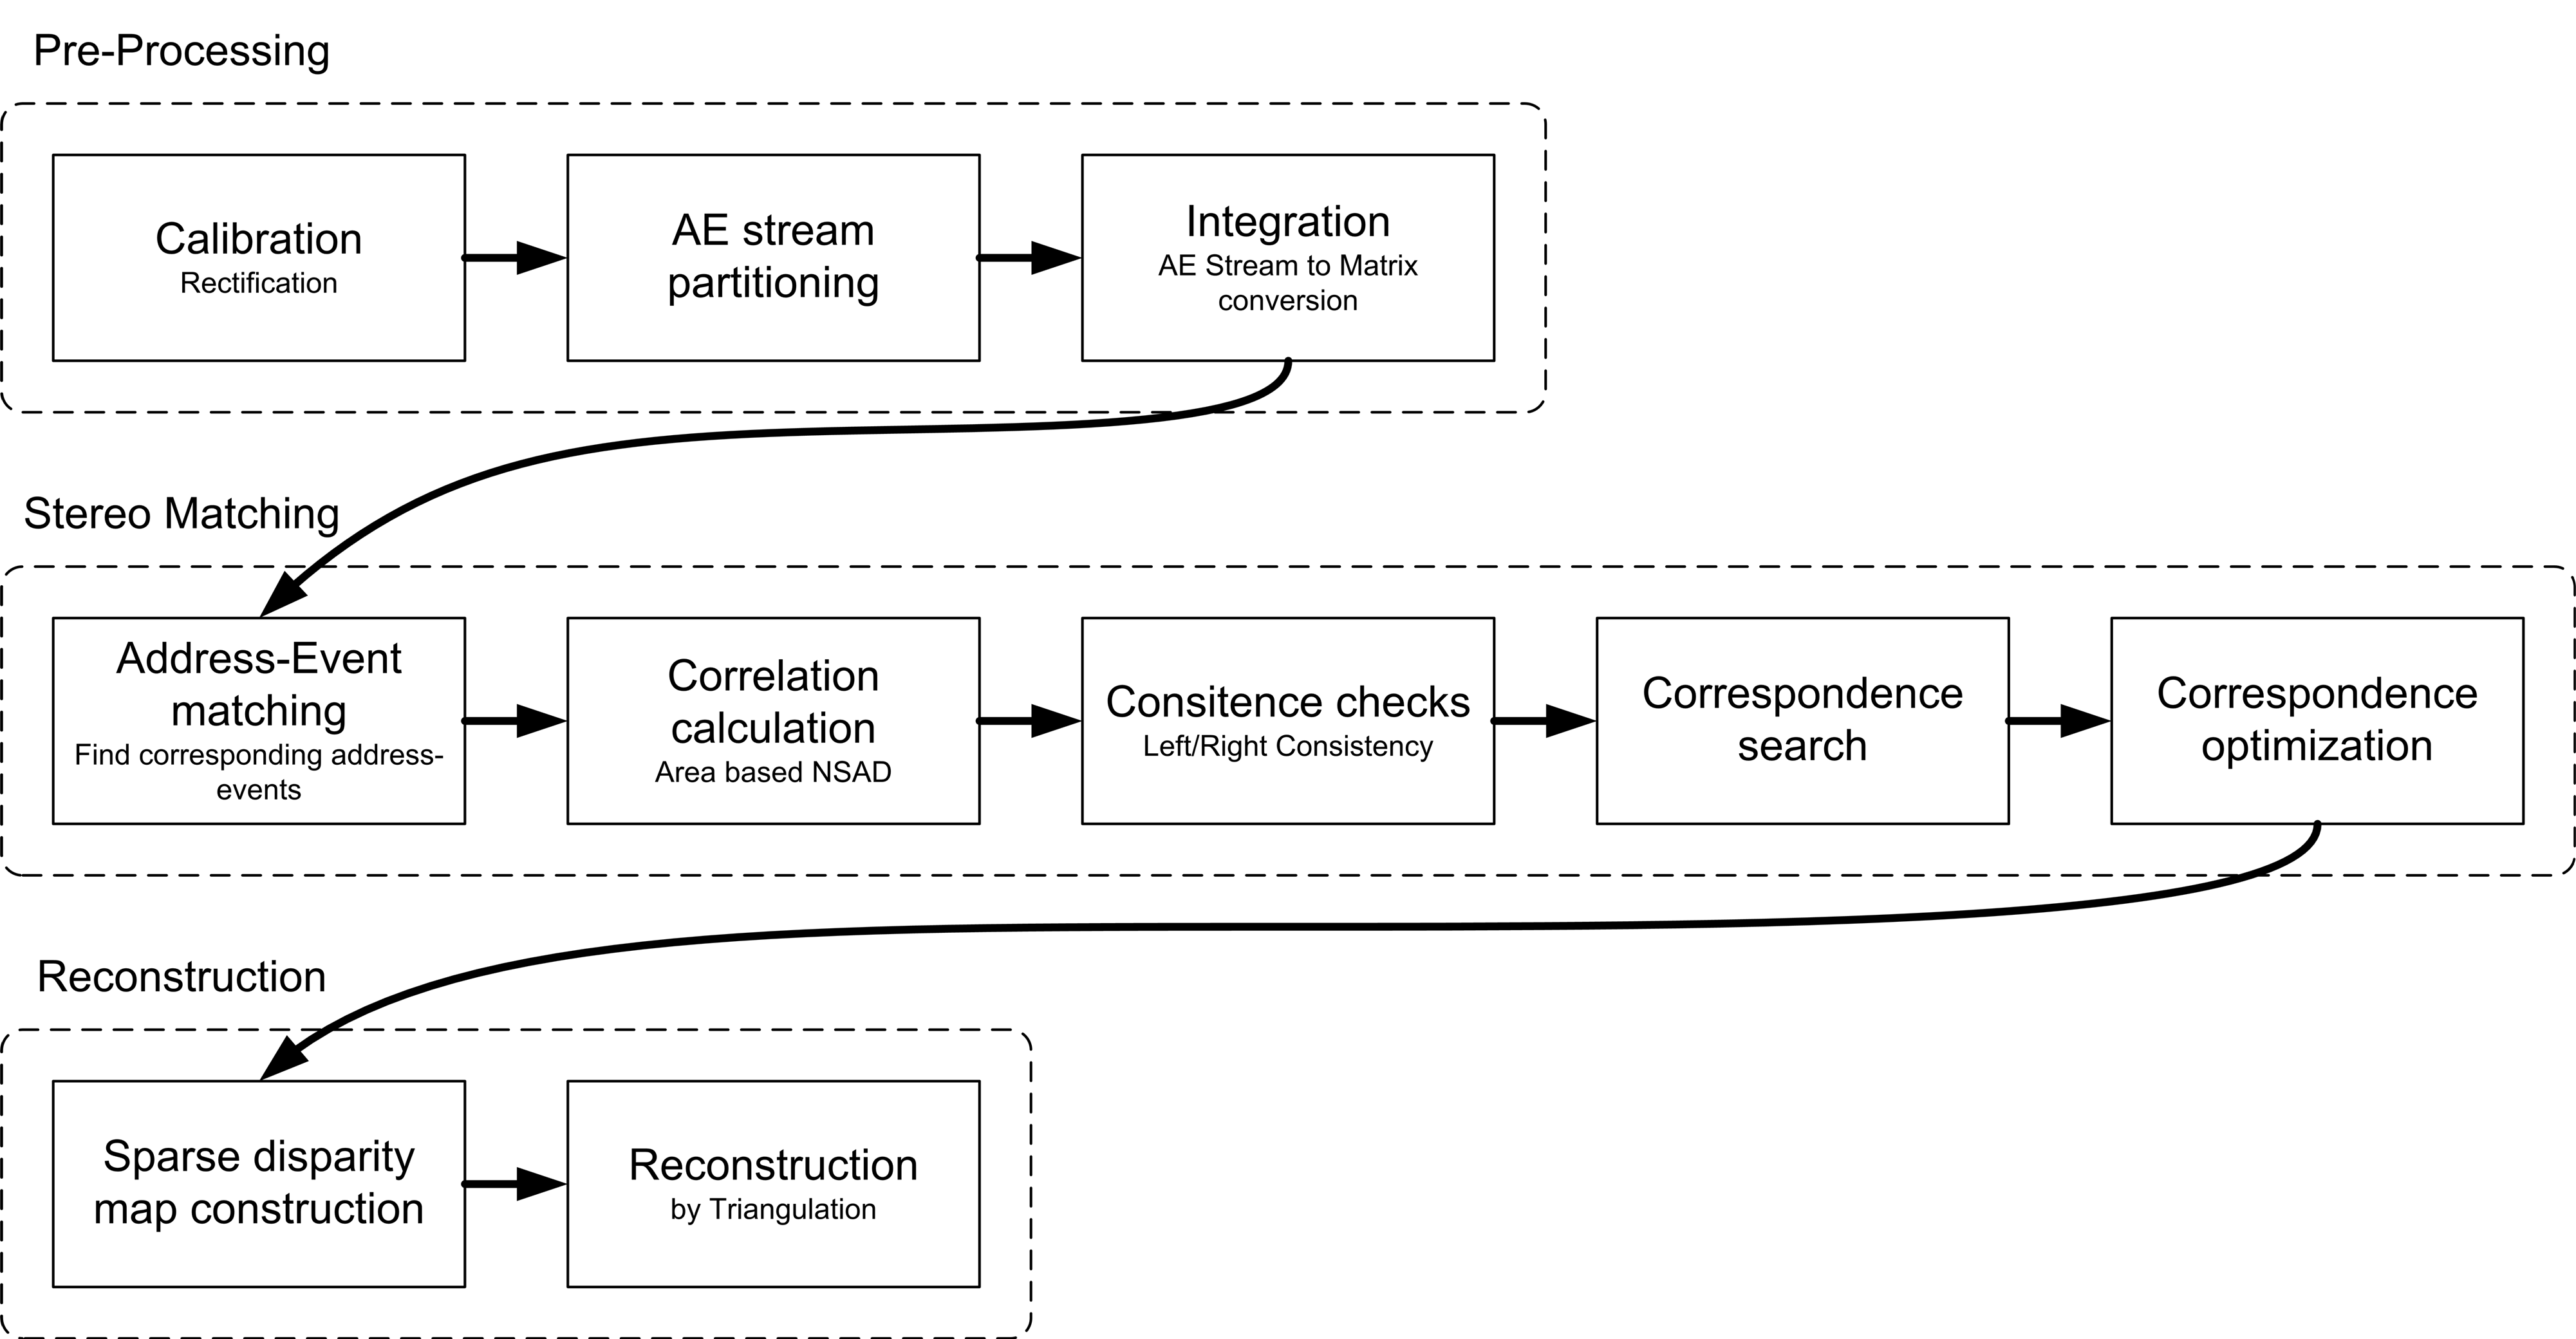
\includegraphics[height=60mm]{Images/DVS_stereo.png}
	\end{center}
	\caption{A block diagram that shows the stereo matching algorithm in \citet{Belbachir01}}
	\label{fig:DVS_stereo}
\end{figure}

In the stereo matching phase, potential matches are searched and the matching cost for all possibles matches is calculated. This is done from both sides to assure constistency. Actually matching events are found by minimizing the earlier calculated cost. 

The distance between matching pixels is put into a disparity map which shows all found events with corresponding distances. 

\section{Approach}
On the basis of DVS and the mentioned stereo matching algorithm, a system can be designed that enables efficient object tracking in three dimension with limited resources. Events can be extracted from a stream of images by comparing consecutive images and remembering pixel positions with changing intensity. The resulting events can be processed in the same way as describe above. A usual image sensor already delivers whole frames which means that there is no need for the stream partitioning step. The rest of the steps don't depend on the choice of the sensor. 

Research can be done for the correlation calculation block as there are several algorithms for this step with different characteristics. Consistency may or may not be necessary and there may exist less resource-intensive ways to ensure consistent results. 

In order to demonstrate the capabilities of the system, the disparity map can be used to track an object and measure its path. Accuracy of the path displays the effectiveness of the system while resource usage gives a measure of the efficiency of the designed system. 